\documentclass{article}

\usepackage{url} 
\usepackage{geometry,afterpage}
\usepackage{pdfpages}
\usepackage{lastpage}
\usepackage{fancyhdr}
\usepackage{ngerman}
\usepackage{listings}

\usepackage{floatrow}
\usepackage[tableposition=top]{caption}
\floatsetup[table]{capposition=top}

\usepackage{multicol}

\usepackage{amsmath, amssymb}

\usepackage[utf8]{inputenc}


\usepackage[numbib]{tocbibind}



\newcommand\twodigits[1]{%
   \ifnum#1<10 0#1\else #1\fi
}



\lhead{Beta Absorption}
\rhead{\today \\ J. Winkler}
%\cfoot{\twodigits{\thepage}~/ \pageref{LastPage}}
\cfoot{{\thepage}~/ \pageref{LastPage}}

\begin{document}

\parindent0cm


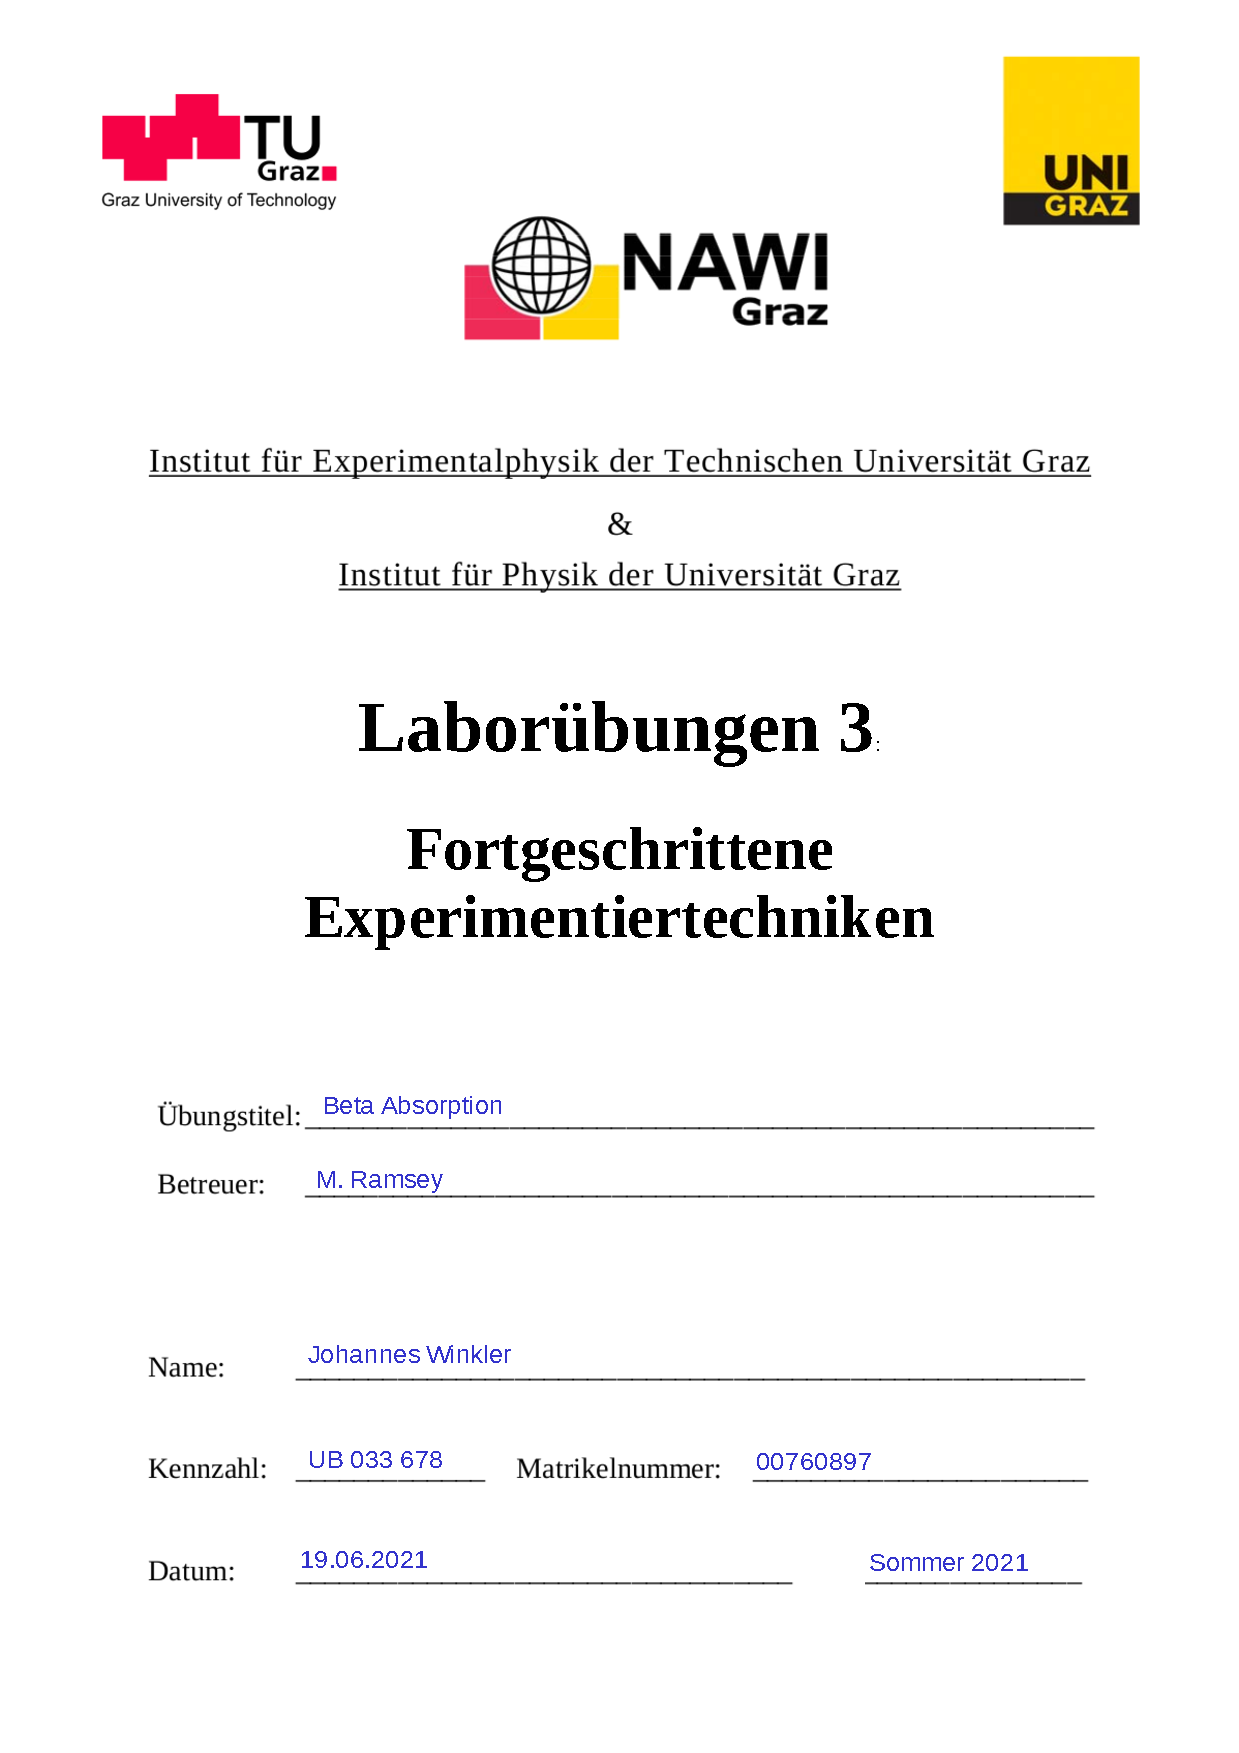
\includepdf{Deckblatt_neu_custom.pdf}


\pagestyle{fancy}

\section{Aufgabenstellung}

Die für das Experiment nötigen Daten inklusive der Aufgabenstellung wurden zur Verfügung gestellt. 

\begin{enumerate}
\item Bestimmung der Hintergrundstrahlung
\item Messung der Absorption der $\beta$-Strahlung durch Aluminium- bzw Kupferfolien in Abhängigkeit von der Massendicke $\rho_d$
\item Bestimmung man den Massenabsorptions-Koeffizienten und die maximale Energie $E_0$ der $\beta$-Teilchen für Aluminium und Kupfer
\item Bestimmung der effektiven Reichweite und den Wert $E$ der mit $E_0$ verglichen werden soll
\end{enumerate}


\section{Grundlagen}

Die Absorptionskurve zeigt einen exponentiellen Abfall bezüglich der Dicke $d$. Dieser ist gegeben durch
\begin{align}
\frac{I}{I_0} = e^{-\mu\cdot d}
\label{eq:absorb}
\end{align}
wobei $\mu$ der Absorptionskoeffizient ist. $E_0$ kann anhand der empirischen Formel
\begin{align}
\frac{\mu}{\rho} = \dfrac{17}{E_0^{1.14}}
\label{eq:E0}
\end{align}
berechnet werden. Bei bekannter effektiver Reichweite kann $E_0$ auch durch die Formel
\begin{align}
R_\text{eff} = 0.412\cdot E_0^{1.38}
\label{eq:Reff}
\end{align}
berechnet werden.

%\begin{figure}[H]
%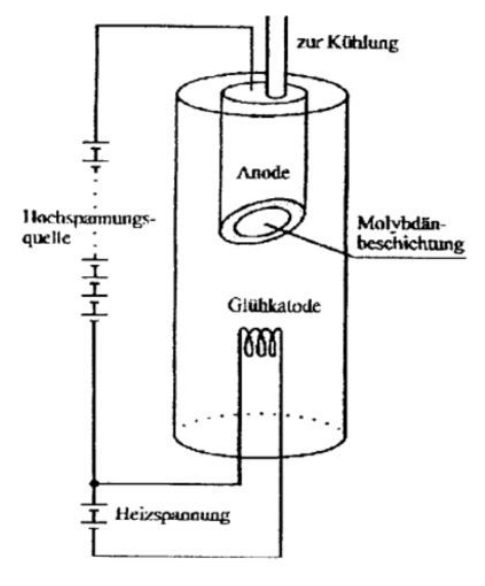
\includegraphics[scale=1.8]{roehre.png}
%\caption{Der schematische Aufbau einer Röntgenröhre. In der Glühkathode werden Elektronen beschleunigt. Diese werden an der Anode abgebremst. Dadurch entsteht Röntgenstrahlung.}
%\label{fig:roentgenroehre}
%\end{figure}






\section{Versuchsaufbau}


\begin{figure}[H]
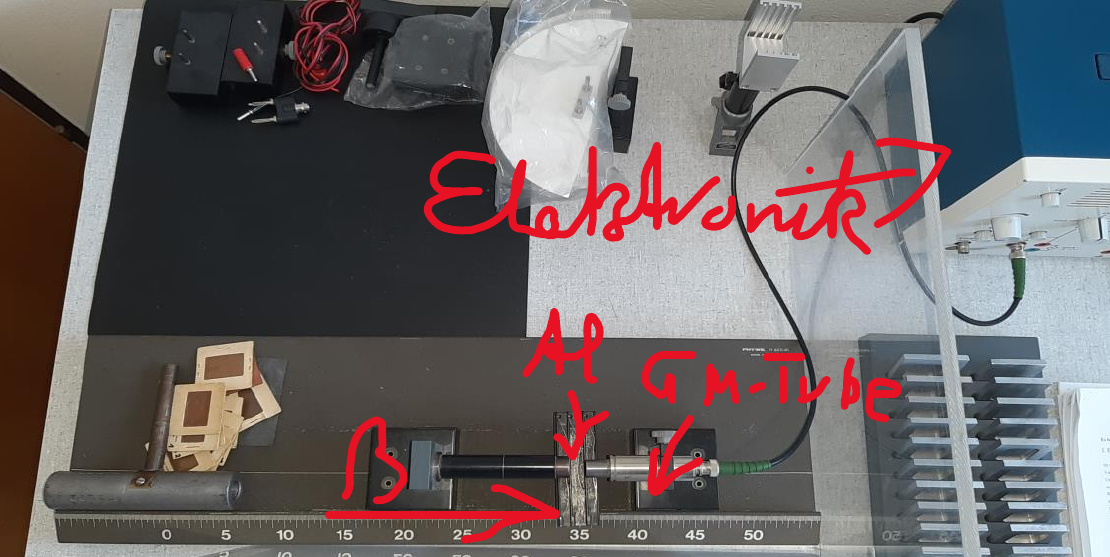
\includegraphics[scale=0.5]{aufbau.png}
\caption{Versuchsanordnung gemäß Skriptum \cite{moodle}.}
\end{figure}

\begin{figure}[H]
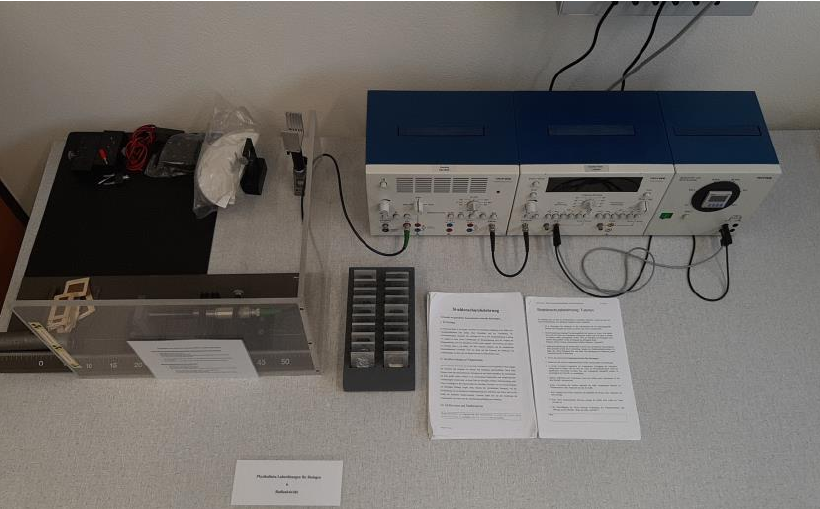
\includegraphics[scale=1]{aufbau2.png}
\caption{Arbeitsplatz gemäß Skriptum \cite{moodle}.}
\end{figure}



\section{Geräteliste}


\begin{table}[H]
\caption{Liste der verwendeten Geräte}

~

\begin{tabular}{l|l}
&Bezeichnung   \\
\hline
1. & Radioaktives Präparat \\
2. & Präparathalterung \\
3. & Halterung für Aluminiumplatten \\
4. & Aluminiumplatten verschiedener Dicke \\
5. & Zählrohr \\
6. & Versorgungsgerät für das Zählrohr \\
7. & Zähler mit Stoppuhr
\end{tabular}

\end{table}


\newpage

\section{Durchführung und Messergebnisse}

Der Versuch wurde wie im Skriptum beschrieben durchgeführt. Die Messwerte wurden bereits im Moodle in einer Excel-Tabelle zur Verfügung gestellt.

Zuerst wurde für 60 Minuten die kosmische Hintergrundstrahlung bestimmt. Diese ergab $N=1292$ mit $\Delta N = \sqrt{1292}$ (Poisson-Verteilung).


\begin{multicols}{2}


\begin{table}[H]
\caption{Messwerte Aluminium bei einer Plattendicke $d$ mit $\Delta d = 0.05$~mm, mit der Messdauer $t$ und $\Delta t=1$~s und der Anzahl der Impulse $N$ mit $\Delta N = \sqrt{n}$ nach Poisson-Verteilung.}

\begin{tabular}{cc}
\end{tabular}
\begin{tabular}{rrr}
$d$ / mm & $t$ / min & N \\
\hline
0.0 & 2 & 175641 \\
0.1 & 4 & 253232 \\
0.2 & 4 & 177828 \\
0.3 & 5 & 107797 \\
0.4 & 10 & 256730 \\
0.5 & 10 & 217737 \\
0.6 & 10 & 177992 \\
0.7 & 10 & 159462 \\
0.8 & 10 & 126138 \\
0.9 & 10 & 108890 \\
1.0 & 10 & 94577 \\
1.5 & 15 & 57476 \\
2.0 & 15 & 21771 \\
2.5 & 15 & 7465 \\
3.0 & 15 & 2993 \\
3.5 & 15 & 1824 \\
4.0 & 15 & 1580 \\
4.5 & 15 & 1560 \\
5.0 & 15 & 1419 \\
5.5 & 25 & 2260 \\
6.0 & 45 & 4258 
\end{tabular}
\end{table}

\columnbreak


\begin{table}[H]
\caption{Messwerte Kupfer bei einer Plattendicke $d$ mit $\Delta d = 0.05$~mm, mit der Messdauer $t$ und $\Delta t=1$~s und der Anzahl der Impulse $N$ mit $\Delta N = \sqrt{n}$ nach Poisson-Verteilung.}

\begin{tabular}{cc}
\end{tabular}
\begin{tabular}{rrr}
$d$ / mm & $t$ / min & N \\
\hline
0.0 & 2 & 167218\\
0.1 & 3 & 46370\\
0.2 & 6 & 50479\\
0.3 & 10 & 44080\\
0.4 & 10 & 25153\\
0.5 & 10 & 10750\\
0.6 & 15 & 8616\\
0.7 & 30 & 7863\\
0.8 & 30 & 4763\\
0.9 & 30 & 3253\\
1.0 & 30 & 2648\\
1.5 & 30 & 2134\\
2.0 & 40 & 2710
\end{tabular}
\end{table}

\end{multicols}

\newpage


\section{Auswertung}


Zuerst wurden in Grafik~\ref{fig:al_imp} und \ref{fig:al_imp_log} der Zusammenhang zwischen der Dicke und den Impulsen pro Sekunde visualisiert. Analog auch für Kupfer in den Grafiken \ref{fig:cu_imp} und \ref{fig:cu_imp_log}


\begin{figure}[H]
\centering
\includegraphics[scale=0.6]{Al_imp.png}
\caption{Impulse pro Sekunde bei Aluminium abhängig von der Dicke.}
\label{fig:al_imp}
\end{figure}

\begin{figure}[H]
\centering
\includegraphics[scale=0.6]{Al_imp_log.png}
\caption{Impulse pro Sekunde bei Aluminium abhängig von der Dicke mit Logarithmischer Skalierung der $y$-Achse}
\label{fig:al_imp_log}
\end{figure}








\begin{figure}[H]
\centering
\includegraphics[scale=0.6]{Cu_imp.png}
\caption{Impulse pro Sekunde bei Kupfer abhängig von der Dicke. }
\label{fig:cu_imp}
\end{figure}





\begin{figure}[H]
\centering
\includegraphics[scale=0.6]{Cu_imp_log.png}
\caption{Impulse pro Sekunde bei Kupfer abhängig von der Dicke mit Logarithmischer Skalierung der $y$-Achse}\label{fig:cu_imp_log}
\end{figure}



\newpage

Als nächstes wird die Masse pro Flächeneinheit abhängig von der Dichte ausgerechnet. Dazu wurden die Dichten in \cite{demtroeder} recherchiert. Es gilt
\begin{align*}
\rho_{\text{Al}} &= 2700~\text{kg} \cdot \text{m}^{-3}\\
\rho_{\text{Cu}} &= 8960~\text{kg} \cdot \text{m}^{-3}
\end{align*}

Für die Masse bezogen auf eine Flächeneinheit des Materials gilt abhängig von der Dichte $d$
\begin{align*}
\rho_d = \rho\cdot d
\end{align*}




\begin{table}[H]
\caption{Für Aluminium: Masse bezogen auf Flächeninhalt $\rho_d$ abhängig von der Dicke $d$ und Impulse pro Sekunde (nach Abzug der Hintergrundstrahlung). }
\begin{tabular}{rrrr}
$d$ / mm & $\rho_d$ / $\dfrac{\text{mg}}{\text{cm}^3}$ & $I$ / s$^{-1}$ & $\Delta I$ / s$^{-1}$ \\
\hline
0.0      &      0        &      1463     &      38 \\
0.1      &      27       &      1055     &      32 \\
0.2      &      54       &      741      &      27 \\
0.3      &      81       &      359      &      19 \\
0.4      &      108      &      428      &      21 \\
0.5      &      135      &      363      &      19 \\
0.6      &      162      &      296      &      17 \\
0.7      &      189      &      265      &      16 \\
0.8      &      216      &      210      &      14 \\
0.9      &      243      &      181      &      13 \\
1.0      &      270      &      157      &      13 \\
1.5      &      405      &      64       &      8 \\
2.0      &      540      &      24       &      5 \\
2.5      &      675      &      8        &      3 \\
3.0      &      810      &      3        &      2 \\
3.5      &      945      &      2        &      1 \\
4.0      &      1080     &      1        &      1 \\
4.5      &      1215     &      1        &      1 \\
5.0      &      1350     &      1        &      1 \\
5.5      &      1485     &      1        &      1 \\
6.0      &      1620     &      1        &      1 
\end{tabular}
\end{table}


\begin{table}[H]
\caption{Für Kupfer: Masse bezogen auf Flächeninhalt $\rho_d$ abhängig von der Dicke $d$ und Impulse pro Sekunde (nach Abzug der Hintergrundstrahlung).}
\begin{tabular}{rrrrrr}
$d$ / mm & $\rho_d$ / $\dfrac{\text{mg}}{\text{cm}^3}$ & $I$ / s$^{-1}$ & $\Delta I$ / s$^{-1}$ \\
\hline
0.0      &      0        &      1393     &      37 \\
0.1      &      90       &      257      &      16 \\
0.2      &      179      &      140      &      12 \\
0.3      &      269      &      73       &      9 \\
0.4      &      358      &      42       &      6 \\
0.5      &      448      &      18       &      4 \\
0.6      &      538      &      9        &      3 \\
0.7      &      627      &      4        &      2 \\
0.8      &      717      &      2        &      2 \\
0.9      &      806      &      1        &      1 \\
1.0      &      896      &      1        &      1 \\
1.5      &      1344     &      1        &      1 \\
2.0      &      1792     &      1        &      1 
\end{tabular}
\end{table}



Aus Formel~\eqref{eq:absorb} erhält man durch Logarithmieren und Erweitern
\begin{align*}
\operatorname{ln}(I) -\operatorname{ln}(I_0) = -\frac{\mu}{\rho} \cdot \left(\rho \cdot d\right)
\end{align*}
sodass man einen linearen Zusammenhang mit Steigung $\mu/\rho$ erkennen kann. Diesen linearen Zusammenhang kann man in den Grafiken~\ref{fig:al_imp_log} und \ref{fig:cu_imp_log} erkennen. Durch eine Regression im linearen Bereich erhält man $\mu/\rho$. Der Vorteil hierbei ist, dass beim Logarithmieren das $I_0$ nicht berücksichtigt werden muss, da dieses die Regressionsgerade nur in der Höhe verschiebt und die Steigung nicht beeinflusst.

Die Regressionsgeraden wurden mit den entsprechenden Stützstellen in den Grafiken~\ref{fig:al_imp_log_regr} und \ref{fig:cu_imp_log_regr} dargestellt. Der Massenabsorptions-Koeffizient ist dann jeweils
\begin{align*}
\frac{\mu_{\text{Al}}}{\rho_{\text{Al}}} &= (7.07 \pm 0.60)~\text{cm}^2~\text{g}^{-1} \\
\frac{\mu_{\text{Cu}}}{\rho_{\text{Cu}}} &= (7.51 \pm 0.57)~\text{cm}^2~\text{g}^{-1}
\end{align*}



\begin{figure}[H]
\centering
\includegraphics[scale=0.6]{Al_imp_log_regression_converted_x.png}
\caption{Impulse pro Sekunde bei Aluminium abhängig von der Massendicke mit Logarithmischer Skalierung der $y$-Achse mit linearer Approximation.}
\label{fig:al_imp_log_regr}
\end{figure}


\begin{figure}[H]
\centering
\includegraphics[scale=0.6]{Cu_imp_log_regression_converted_x.png}
\caption{Impulse pro Sekunde bei Kupfer abhängig von der Massendicke mit Logarithmischer Skalierung der $y$-Achse mit linearer Approximation.}
\label{fig:cu_imp_log_regr}
\end{figure}

Daraus folgt aus Gleichung~\eqref{eq:E0}
\begin{align*}
E_{0,\text{Al}} &= (2.16\pm0.53)~\text{MeV}\\ 
E_{0,\text{Cu}} &= (2.04\pm0.48)~\text{MeV}
\end{align*}



Die effektive Reichweite $R_\text{eff}$ folgt dann durch Extrapolation 
\begin{align*}
R_{\text{eff},\text{Al}} &= (975.29\pm 18.23)~\text{mg}/\text{cm}^2 \\
R_{\text{eff},\text{Cu}} &= (835.39\pm 15.07)~\text{mg}/\text{cm}^2 
\end{align*}


Aus der effektiven Reichweite kann auch mit Gleichung \eqref{eq:Reff} berechnet werden
\begin{align*}
E_{0,\text{Al}} &= (1.86 \pm 0.23)~\text{MeV} \\ 
E_{0,\text{Cu}} &= (1.67 \pm 0.15)~\text{MeV}
\end{align*}




\section{Diskussion und Zusammenfassung}

Es wurde die Konstante $\mu/\rho$ im exponentiellen Abfall
\begin{align*}
I = I_0\cdot \exp\left(-\frac{\mu}{\rho} \cdot (\rho\cdot d)\right) 
\end{align*}
berechnet. Da bei den Messungen Unregelmäßigkeiten auftreten können, ist dieses Ergebnis nicht ganz genau. Bei der Aluminiumfolie ist ein Knick in der Kurve zu sehen. Dies deutet auf einen Messfehler hin. Außerdem erkennt man den exponentiellen Teil durch die Linearität beim Logarithmieren. Da der exponentielle Teil händisch durch Ablesen gefunden wurde, existiert hier eine zusätzliche Fehlerquelle.

Die gefundenen Energien für den Massenabsorptionskoeffizient sind
\begin{align*}
E_{0,\text{Al}} &= (2.16\pm0.53)~\text{MeV}\\ 
E_{0,\text{Cu}} &= (2.04\pm0.48)~\text{MeV}
\end{align*}
während die Energien durch die effektive Reichweite 
\begin{align*}
E_{0,\text{Al}} &= (1.86 \pm 0.23)~\text{MeV} \\ 
E_{0,\text{Cu}} &= (1.67 \pm 0.15)~\text{MeV}
\end{align*}
sind. Da die Differenz zwischen den beiden gleich groß ist, könnte es einen systematischen Fehler geben. 

\begin{thebibliography}{9}
\bibitem{moodle} S. Surnev: Skript zur Beta-Absorption aus dem Moodle der Karl-Franzens Universität, Institut für Physik, 15.06.2021.
\bibitem{daten} S. Surnev: Daten zur Röntgenbeugung aus dem Moodle der Karl-Franzens Universität, Institut für Physik, 26.04.2021.
\bibitem{messmethoden}  R. Dämon: Einführung in die physikalischen Messmethoden, Graz 2016.
\bibitem{demtroeder}  W. Demtröder: Experimentalphysik 1.
\end{thebibliography}


\newpage 
\appendix

%\section{Python Skript}



\definecolor{commentgreen}{RGB}{2,112,10}
\definecolor{eminence}{RGB}{108,48,130}
\definecolor{weborange}{RGB}{255,165,0}
\definecolor{frenchplum}{RGB}{129,20,83}

\lstdefinelanguage{python}{
    morekeywords={def, for, range, abs, return},
    otherkeywords={<-,->, |>, \%\{, \}, \{, \, (, )},
    sensitive=true,
    morecomment=[l]{\#},
    morecomment=[n]{/*}{*/},
    morecomment=[s][\color{purple}]{:}{\ },
    morestring=[s][\color{orange}]"",
    commentstyle=\color{commentgreen},
    keywordstyle=\color{eminence},
    stringstyle=\color{red},
	basicstyle=\ttfamily,
	breaklines,
	showstringspaces=false,
	frame=tb
}
%\lstinputlisting[language=Python,captionpos=b, label=lst:test,caption={Laplace Auswertung}]{generate_numbers_laplace.py}

%\lstinputlisting[language=Python,captionpos=b, label=lst:test,caption={Bessel Auswertung}]{generate_numbers_bessel.py}



\end{document}